\subsection*{4.4.1. Chi tiết kỹ thuật OCR hóa đơn: mô hình, huấn luyện và đánh giá}
\addcontentsline{toc}{subsection}{4.4.1. Chi tiết kỹ thuật OCR hóa đơn: mô hình, huấn luyện và đánh giá}
Mục này trình bày thành phần AI/OCR dùng để số hóa hóa đơn trong phân hệ Kho – Mua sắm: kiến trúc dịch vụ, cơ sở lý thuyết các mô hình, quá trình huấn luyện trên dữ liệu tự sinh và kết quả đánh giá – so sánh giữa các engine. Đây là phần đóng góp kỹ thuật của tác giả cho phân hệ.

\subsubsection*{a) Kiến trúc dịch vụ OCR đa engine}
Dịch vụ OCR viết bằng Python/FastAPI, tách khỏi backend .NET và gọi qua HTTP (POST /extract). Nhận dạng chạy bất đồng bộ: mỗi yêu cầu vào hàng đợi (OcrJobQueue) và một tiến trình nền (OcrProcessingWorker) lấy ra xử lý, nhờ đó giao diện không phải chờ. Dịch vụ cài đặt \textbf{ba engine OCR tự chủ}, người dùng chọn trên giao diện (lưu ở \texttt{ocr\_jobs.ocrEngine}): \texttt{paddleocr} (mặc định), \texttt{vietocr} (EasyOCR phát hiện + VietOCR nhận dạng) và biến thể lai \texttt{paddledet\_viet} (DBNet của Paddle phát hiện + VietOCR nhận dạng). Dù dùng engine nào, kết quả cũng quy về cấu trúc dòng chuẩn hóa [\{text, box, prob\}] rồi đưa vào chung một hàm bóc tách trường, nên việc đổi engine không ảnh hưởng khâu lấy trường.

\begin{center}{\singlespacing\renewcommand{\arraystretch}{1.25}
\begin{tabular}{|>{\raggedright\arraybackslash}p{\dimexpr\linewidth/5-2\tabcolsep-\arrayrulewidth\relax}|>{\raggedright\arraybackslash}p{\dimexpr\linewidth/5-2\tabcolsep-\arrayrulewidth\relax}|>{\raggedright\arraybackslash}p{\dimexpr\linewidth/5-2\tabcolsep-\arrayrulewidth\relax}|>{\raggedright\arraybackslash}p{\dimexpr\linewidth/5-2\tabcolsep-\arrayrulewidth\relax}|>{\raggedright\arraybackslash}p{\dimexpr\linewidth/5-2\tabcolsep-\arrayrulewidth\relax}|}
\hline
\textbf{model} & \textbf{Phát hiện (detect)} & \textbf{Nhận dạng (recognize)} & \textbf{Fine-tune} & \textbf{Đặc điểm} \\ \hline
vietocr & EasyOCR (CRAFT) & VietOCR (VGG + Transformer) & recognition & Tự chủ, mạnh về dấu tiếng Việt \\ \hline
paddleocr & PaddleOCR (DBNet) & PP-OCRv4 (SVTR\_LCNet) & detect + recognize & Hợp nhất, nhẹ, fine-tune cả hai tầng \\ \hline
paddledet\_viet & PaddleOCR (DBNet) & VietOCR (VGG + Transformer) & detect + recognition & Hybrid: DBNet mạnh + VietOCR đọc dấu tốt \\ \hline
\end{tabular}}\end{center}
\begin{figure}[htbp]\centering
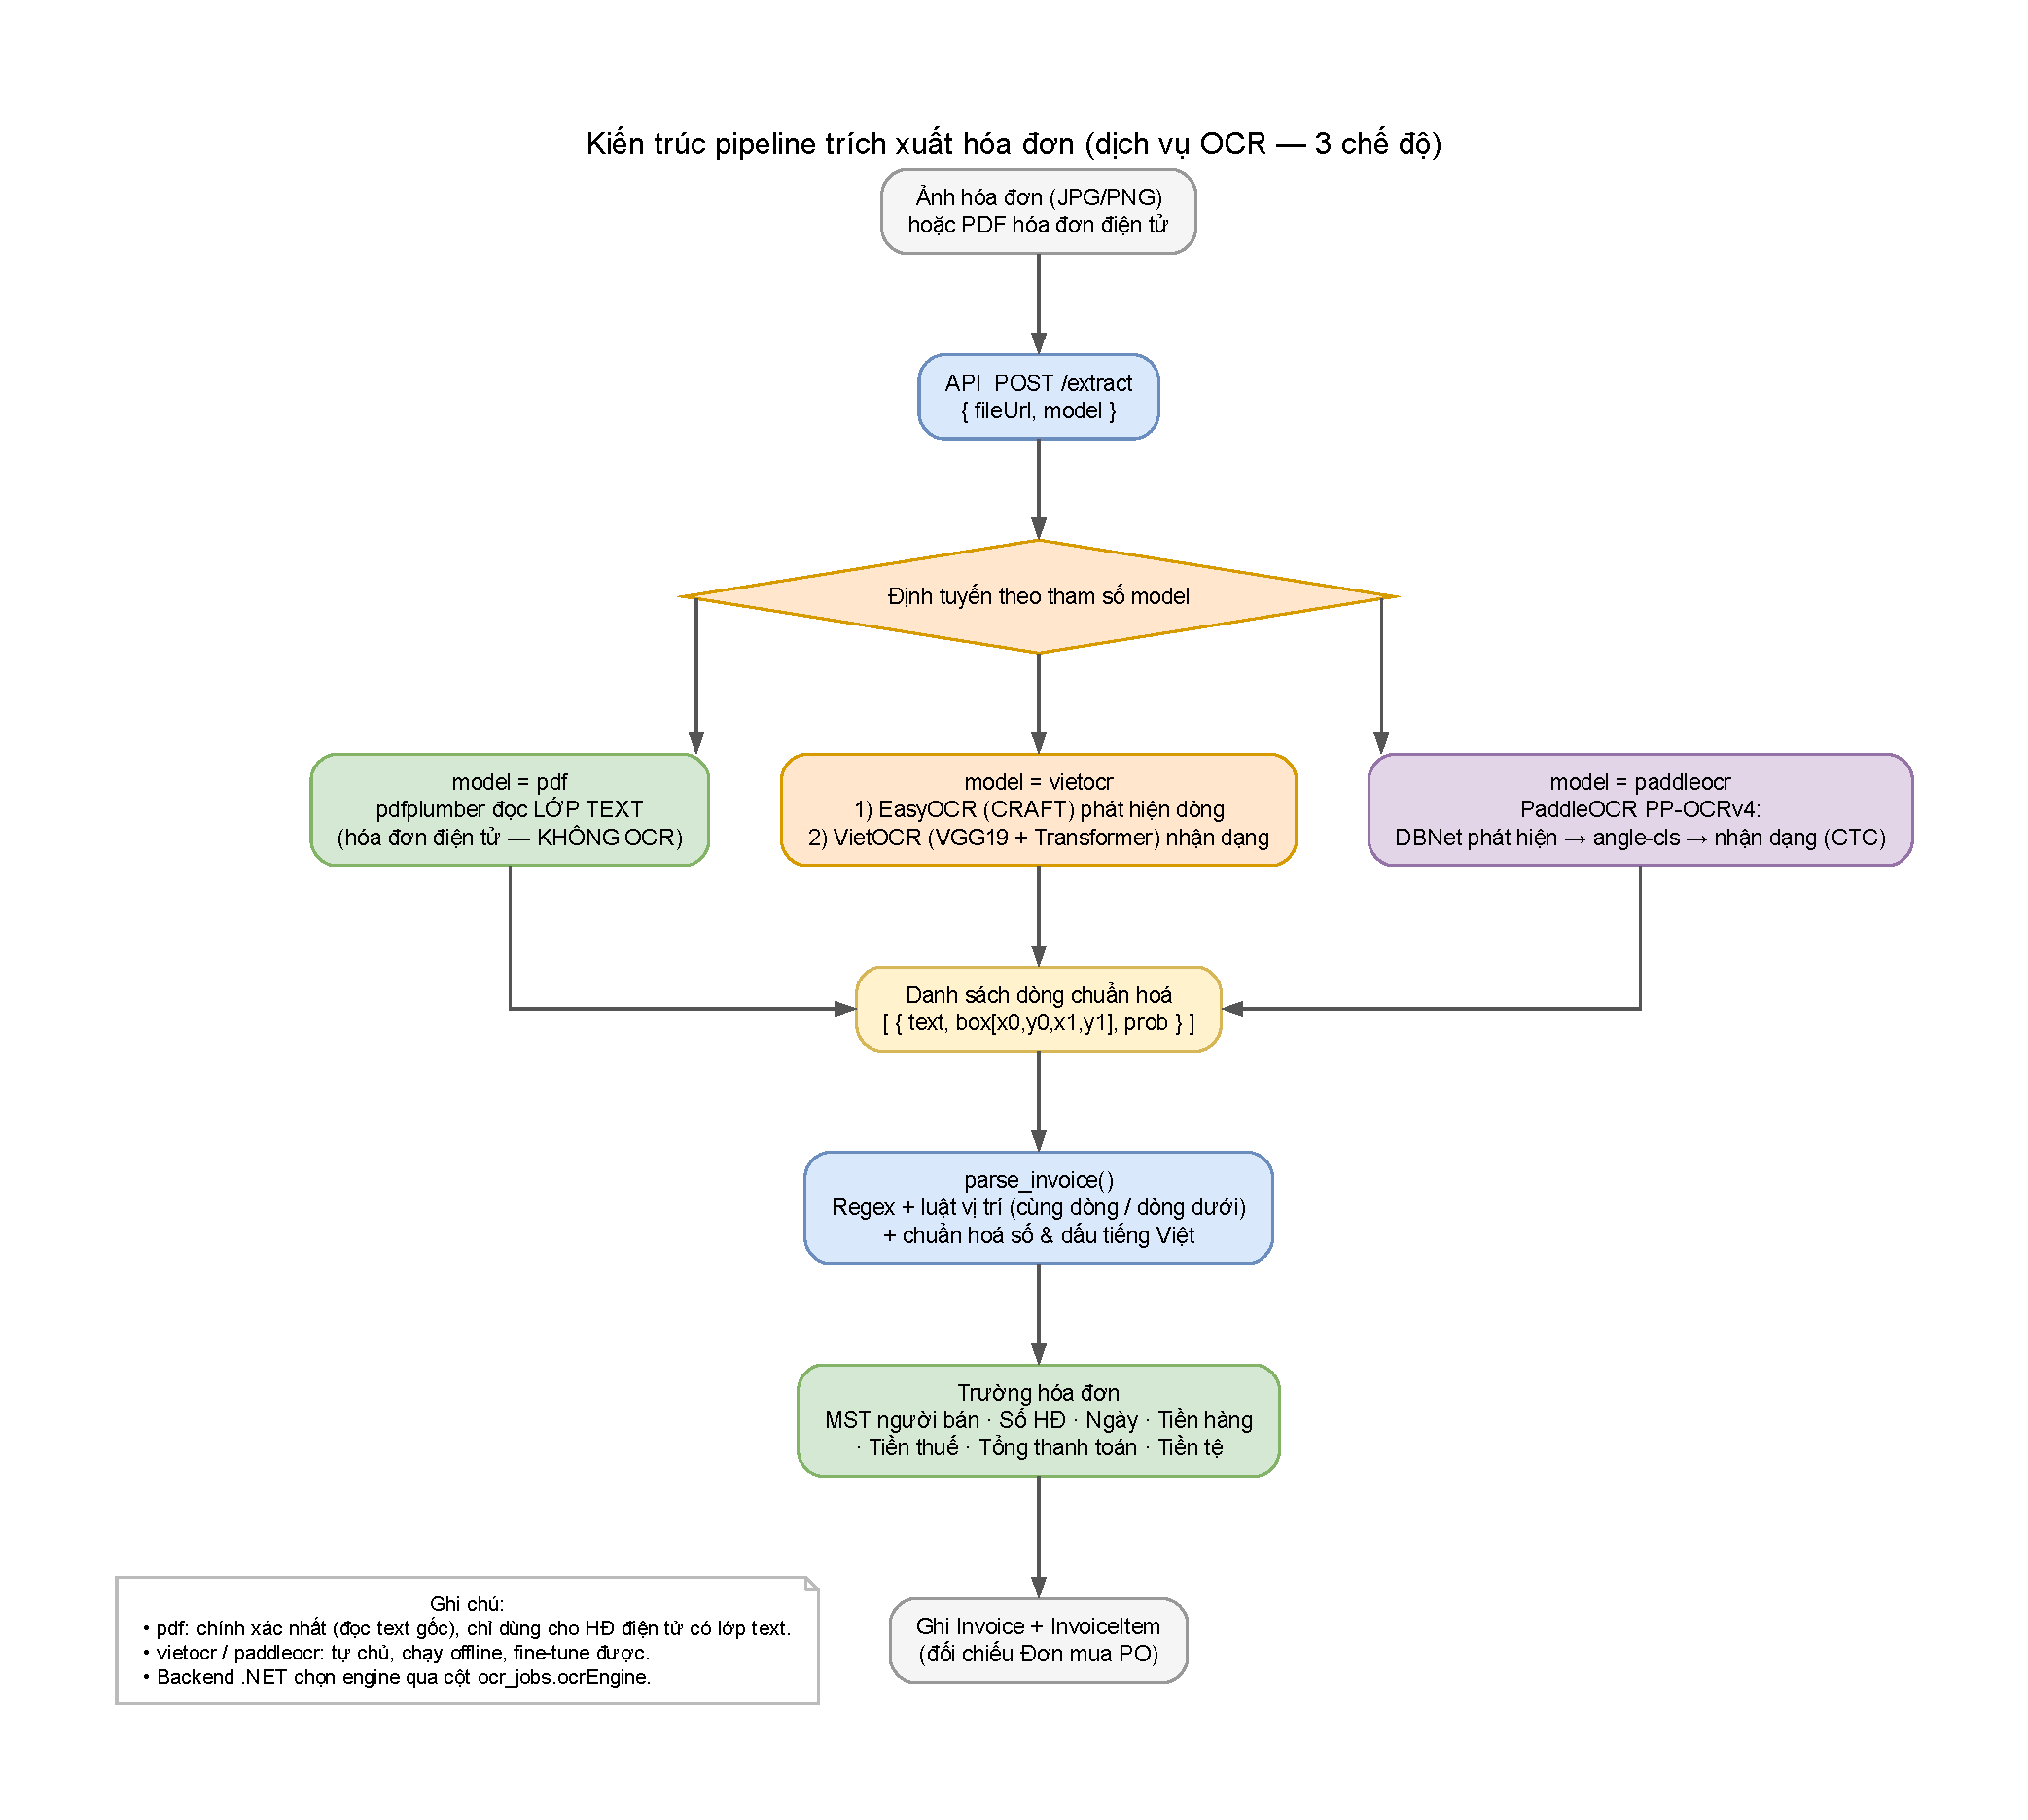
\includegraphics[width=\linewidth,height=0.5\textheight,keepaspectratio]{images/img27.pdf}
\caption*{\small Hình 4.20. Kiến trúc pipeline trích xuất hóa đơn của dịch vụ OCR}
\addcontentsline{lof}{figure}{Hình 4.20. Kiến trúc pipeline trích xuất hóa đơn của dịch vụ OCR}
\end{figure}
\subsubsection*{b) Cơ sở lý thuyết các mô hình}
\textbf{VietOCR} (vgg\_transformer, chỉ nhận dạng): CNN VGG19 trích đặc trưng ảnh dòng rồi Transformer encoder–decoder (seq2seq + attention) sinh từng ký tự theo từ điển tiếng Việt — đọc dấu thanh rất tốt nhưng buộc ghép một bộ phát hiện bên ngoài. \textbf{PaddleOCR} (PP-OCRv4, hợp nhất phát hiện + nhận dạng): DBNet (Differentiable Binarization) tách vùng chữ gọn, phân loại góc xoay dòng, rồi SVTR\_LCNet (huấn luyện GTC = CTC + NRTR) nhận dạng theo bảng ký tự \texttt{dict\_vi.txt} (137 ký tự) — một bộ công cụ, fine-tune được cả hai tầng, nhẹ, chạy offline. \textbf{EasyOCR (CRAFT)}: pipeline \texttt{vietocr} chỉ mượn CRAFT để cắt dòng; vì CRAFT không được fine-tune trên hóa đơn nên trở thành nút cổ chai — cũng là lý do thử biến thể hybrid \texttt{paddledet\_viet} ở mục h.

\subsubsection*{c) Dữ liệu, huấn luyện và luồng xử lý}
Vì không có sẵn dữ liệu hóa đơn thật đã gán nhãn, đề tài tự sinh dữ liệu hóa đơn GTGT tiếng Việt tổng hợp (synthetic): script tự render hóa đơn và tự ghi tọa độ + nội dung từng ô chữ, nên xuất được cả nhãn phát hiện (det) lẫn nhận dạng (rec) mà không cần gán tay, kèm bảng ký tự \texttt{dict\_vi.txt}. Dữ liệu được random đa dạng bố cục và tăng cường cho ``giống thật'' (nền giấy, nghiêng/méo, nhiễu, nén JPEG, dấu mộc đỏ, chữ ký tay); mọi phép biến hình đều kéo theo tọa độ box nên nhãn luôn khớp. Quy mô mặc định 400–500 hóa đơn, chia train/val 90/10; cả hai mô hình đều fine-tune từ trọng số pretrained (transfer learning) để hội tụ nhanh. Cấu hình thật (đọc từ config.yml):

\begin{center}{\small\singlespacing\renewcommand{\arraystretch}{1.3}
\begin{tabular}{|>{\raggedright\arraybackslash}p{\dimexpr0.16\linewidth-2\tabcolsep-\arrayrulewidth\relax}|>{\raggedright\arraybackslash}p{\dimexpr0.35\linewidth-2\tabcolsep-\arrayrulewidth\relax}|>{\raggedright\arraybackslash}p{\dimexpr0.13\linewidth-2\tabcolsep-\arrayrulewidth\relax}|>{\raggedright\arraybackslash}p{\dimexpr0.09\linewidth-2\tabcolsep-\arrayrulewidth\relax}|>{\raggedright\arraybackslash}p{\dimexpr0.27\linewidth-2\tabcolsep-\arrayrulewidth\relax}|}
\hline
\textbf{Mô hình} & \textbf{Thuật toán / Khởi tạo} & \textbf{Epoch} & \textbf{Batch} & \textbf{Optimizer / LR} \\ \hline
VietOCR (rec) & VGG19 + Transformer, từ vgg\_\allowbreak{}transformer & 20\,000 iters & 32 & mặc định VietOCR \\ \hline
PaddleOCR rec & SVTR\_\allowbreak{}LCNet + GTC(CTC+NRTR), từ PP-OCRv4 & 80 & 64 & Adam + Cosine, lr 0,001 \\ \hline
PaddleOCR det & DBNet, từ PP-OCRv4 det & 150 & 8 & lr 0,001 \\ \hline
\end{tabular}}\end{center}
\textbf{Luồng xử lý. }Pipeline vietocr: ảnh $\rightarrow$ EasyOCR/CRAFT phát hiện dòng $\rightarrow$ cắt dòng $\rightarrow$ VietOCR (VGG19 $\rightarrow$ Transformer) $\rightarrow$ text. Pipeline paddleocr: ảnh $\rightarrow$ DBNet $\rightarrow$ phân loại góc $\rightarrow$ SVTR\_LCNet $\rightarrow$ text. Cả hai gộp về danh sách dòng, đưa vào hàm bóc tách trường và ghi Invoice/InvoiceItem để đối chiếu PO.

\textbf{Kết quả huấn luyện PaddleOCR (số thật từ train.log). }Với nhận dạng (rec), loss giảm nhanh về gần 0 quanh bước \textasciitilde{}2\,500, trên tập val accuracy toàn chuỗi đạt 0,9964 (99,64\%) và norm\_edit\_dis 0,9992 tại epoch 41. Với phát hiện (det), hmean tốt nhất trên val chỉ đạt 0,2298 — cho thấy phát hiện bố cục trên dữ liệu synthetic còn yếu; khuyến nghị bổ sung 50–150 hóa đơn thật gán bằng PPOCRLabel, hoặc kết hợp detector pretrain với recognizer đã fine-tune.

\begin{figure}[htbp]\centering
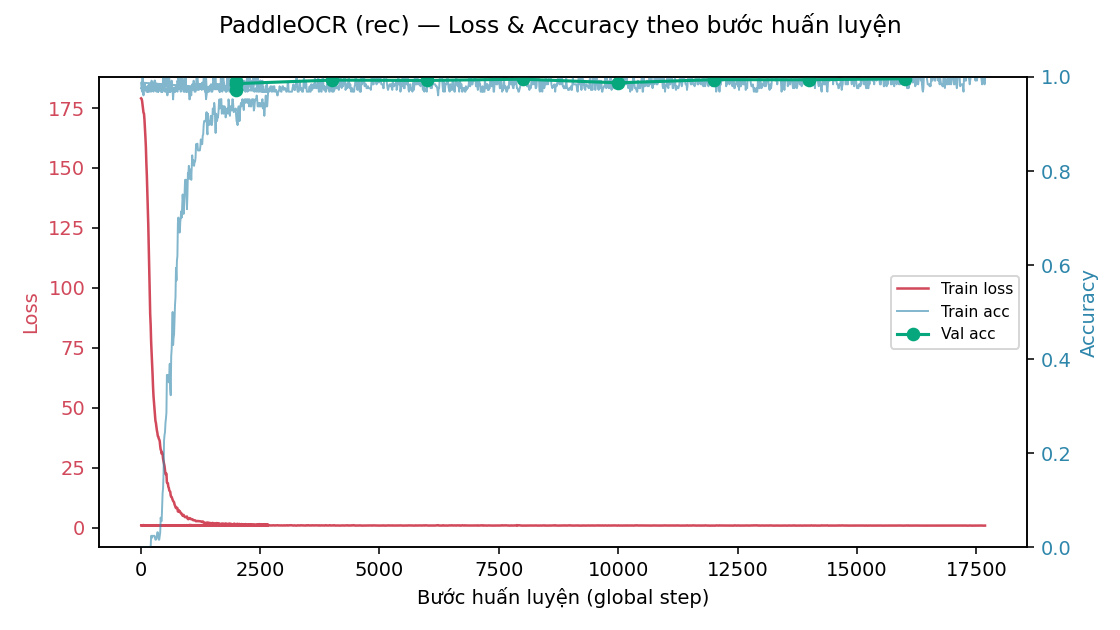
\includegraphics[width=\linewidth,height=0.42\textheight,keepaspectratio]{images/img29.png}
\caption*{\small Hình 4.21. Đường cong huấn luyện PaddleOCR (rec): loss và accuracy theo bước}
\addcontentsline{lof}{figure}{Hình 4.21. Đường cong huấn luyện PaddleOCR (rec)}
\end{figure}
\subsubsection*{d) So sánh và đánh giá ba engine}
Ba engine (EasyOCR, VietOCR, PaddleOCR) được đánh giá trên cùng tập val 300 mẫu với các chỉ số: Seq-acc (đọc đúng toàn chuỗi), Char-acc (1 $-$ CER), NED, CER<0,1 và độ trễ (ms/ảnh, đo trên CPU):

\begin{center}{\small\singlespacing\renewcommand{\arraystretch}{1.25}
\begin{tabular}{|>{\raggedright\arraybackslash}p{\dimexpr0.30\linewidth-2\tabcolsep-\arrayrulewidth\relax}|c|c|c|c|c|}
\hline
\textbf{Cấu hình} & \textbf{Seq-acc} & \textbf{Char-acc} & \textbf{NED} & \textbf{CER<0,1} & \textbf{ms/ảnh} \\ \hline
VietOCR gốc (trước) & 0,870 & 0,976 & 0,977 & 0,903 & - \\ \hline
VietOCR fine-tune (sau) & 1,000 & 1,000 & 1,000 & 1,000 & 317 \\ \hline
PaddleOCR gốc (trước) & 0,463 & 0,882 & 0,882 & 0,513 & - \\ \hline
PaddleOCR fine-tune (sau) & 0,893 & 0,967 & 0,968 & 0,913 & 65 \\ \hline
EasyOCR (baseline) & 0,510 & 0,811 & 0,818 & 0,613 & 156 \\ \hline
Ensemble (bỏ phiếu) & 0,920 & 0,974 & 0,974 & 0,933 & - \\ \hline
Oracle (best-of-3, chặn trên) & 1,000 & - & - & - & - \\ \hline
\end{tabular}}\end{center}
\begin{figure}[htbp]\centering
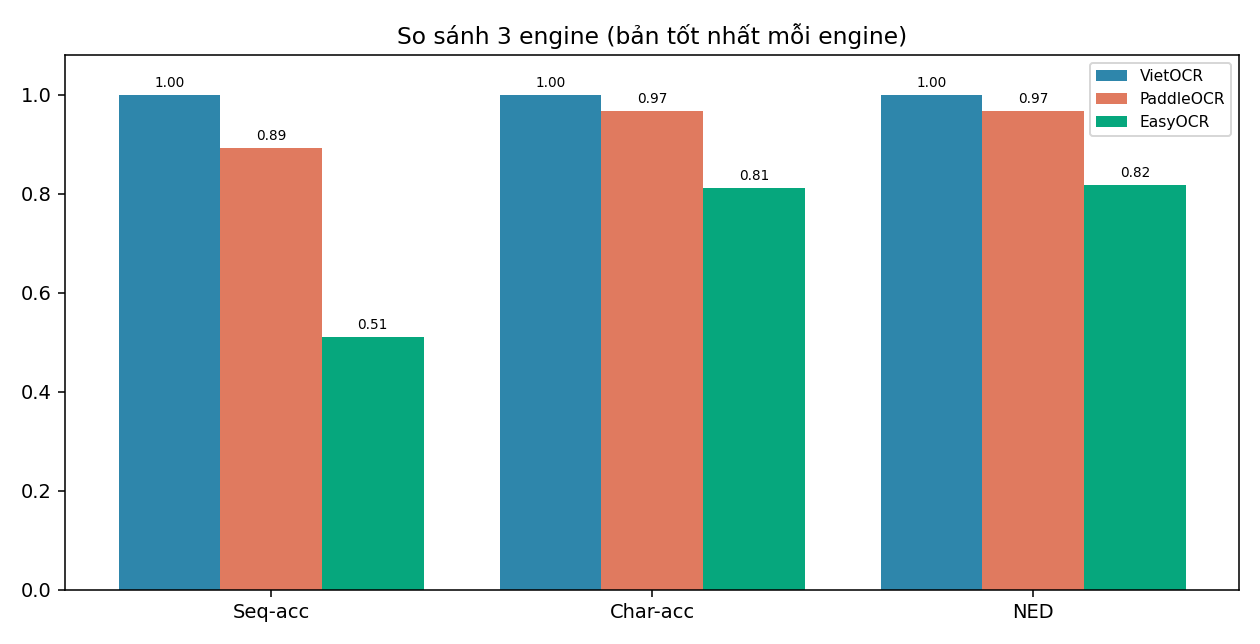
\includegraphics[width=\linewidth,height=0.42\textheight,keepaspectratio]{images/img31.png}
\caption*{\small Hình 4.22. So sánh ba engine theo Seq-acc / Char-acc / NED (tập val 300 mẫu)}
\addcontentsline{lof}{figure}{Hình 4.22. So sánh ba engine theo Seq-acc / Char-acc / NED}
\end{figure}
\textbf{Nhận xét. }(1) Fine-tune có tác động lớn: Seq-acc VietOCR tăng 0,870 $\rightarrow$ 1,000; PaddleOCR tăng 0,463 $\rightarrow$ 0,893 (PaddleOCR gốc pretrain tiếng Trung nên hưởng lợi nhiều nhất). (2) Về độ chính xác nhận dạng, VietOCR fine-tune đứng đầu (đúng 300/300 mẫu), trên PaddleOCR (0,893) và EasyOCR (0,510). (3) Về tốc độ, PaddleOCR nhanh nhất (65 ms/ảnh, nhanh hơn VietOCR \textasciitilde{}4,9 lần) và hợp nhất det+rec. Về \textbf{tính bổ trợ}: trong 300 mẫu không có mẫu nào cả ba cùng sai; ``chỉ VietOCR đúng'' = 24, ``chỉ PaddleOCR/chỉ EasyOCR đúng'' = 0, nên bỏ phiếu ba engine (0,920) còn thấp hơn VietOCR đơn lẻ (1,000) — với bài toán này dùng một engine mạnh hợp lý hơn là bỏ phiếu.

\subsubsection*{e) Lựa chọn mô hình}
\textbf{Vì sao chọn PaddleOCR thay vì kết hợp EasyOCR + VietOCR. }Phương án EasyOCR + VietOCR có recognizer rất chính xác nhưng vướng ba nhược điểm: tầng phát hiện CRAFT không được fine-tune (nút cổ chai), phải nạp hai bộ công cụ (nặng), và chậm nhất (317 ms/ảnh). PaddleOCR là một bộ công cụ hợp nhất, fine-tune được cả DBNet lẫn recognizer trên cùng dataset tự gán nhãn, nhẹ và nhanh nhất (65 ms/ảnh). Vì vậy PaddleOCR được chọn làm engine tự chủ mặc định; VietOCR giữ làm lựa chọn khi cần độ chính xác cao nhất; biến thể hybrid \texttt{paddledet\_viet} kết hợp điểm mạnh hai bên. Toàn bộ đều là giải pháp tự chủ, chạy offline, không phụ thuộc API bên ngoài.

\subsubsection*{f) Thuật toán bóc tách cấu trúc hóa đơn kháng nghiêng (deskew)}
\textbf{Đặt vấn đề. }Tầng OCR chỉ trả về danh sách ô văn bản kèm hộp bao, chưa phải dữ liệu có cấu trúc. Để dựng lại các trường (số hóa đơn, ngày, MST, các dòng tiền) và bảng chi tiết, hệ thống phải gom ô về đúng hàng và cột theo tọa độ. Ảnh chụp điện thoại thường nghiêng vài độ; khi đó độ lệch tung độ giữa mép trái–phải của bảng vượt quá chiều cao một dòng, khiến gom theo y gộp nhầm hai dòng liền kề. Đề tài đề xuất thuật toán hai pha khắc phục bằng hình học – thống kê, chạy sau tầng OCR và không cần huấn luyện.

\textbf{Pha A – Ước lượng và khử nghiêng. }Các ô thuộc hàng tiêu đề bảng (STT, Tên hàng, ĐVT, SL, Đơn giá, Thành tiền) vốn nằm trên cùng một phương ngang. Thuật toán khớp một đường thẳng qua tâm các ô này bằng bình phương tối thiểu; hệ số góc $a$ chính là độ nghiêng ($\theta$ = arctan $a$), rồi áp phép trượt (shear) ngược trên trục tung: $a = \Sigma(x_i - \bar{x})(y_i - \bar{y}) / \Sigma(x_i - \bar{x})^2$ và $y' = y - a\cdot x_i$. Sau đó mọi ô cùng một dòng vật lý có $y'$ xấp xỉ bằng nhau. Nếu $|a| < \varepsilon$ (ảnh vốn thẳng) thì bỏ qua bước trừ, bảo đảm bất biến với ảnh không nghiêng.

\textbf{Pha B – Tái tạo bảng theo cụm tọa độ. }Trên hệ tọa độ đã nắn thẳng: (1) xác định biên bảng giữa hàng tiêu đề và dòng ``Tổng/Thuế''; (2) gom dòng bằng phân cụm một chiều theo $y'$ với ngưỡng 0,6 lần chiều cao dòng trung vị; (3) gán mỗi ô vào cột có tâm hoành độ gần nhất (cột số chọn ô gần tâm cột nhất để tránh dính con số); (4) ghép mỗi cụm thành một dòng hàng và loại dòng rác. Độ phức tạp tổng thể $O(n\log n)$, bộ nhớ $O(n)$ với $n$ là số ô OCR. Trên hóa đơn thử nghiệm bị nghiêng, thuật toán tách đúng 7/7 dòng hàng, trong khi gom theo y thô chỉ nhận 3 hàng do bị dồn — thuần hình học, không cần mạng nơ-ron.

\begin{figure}[htbp]\centering
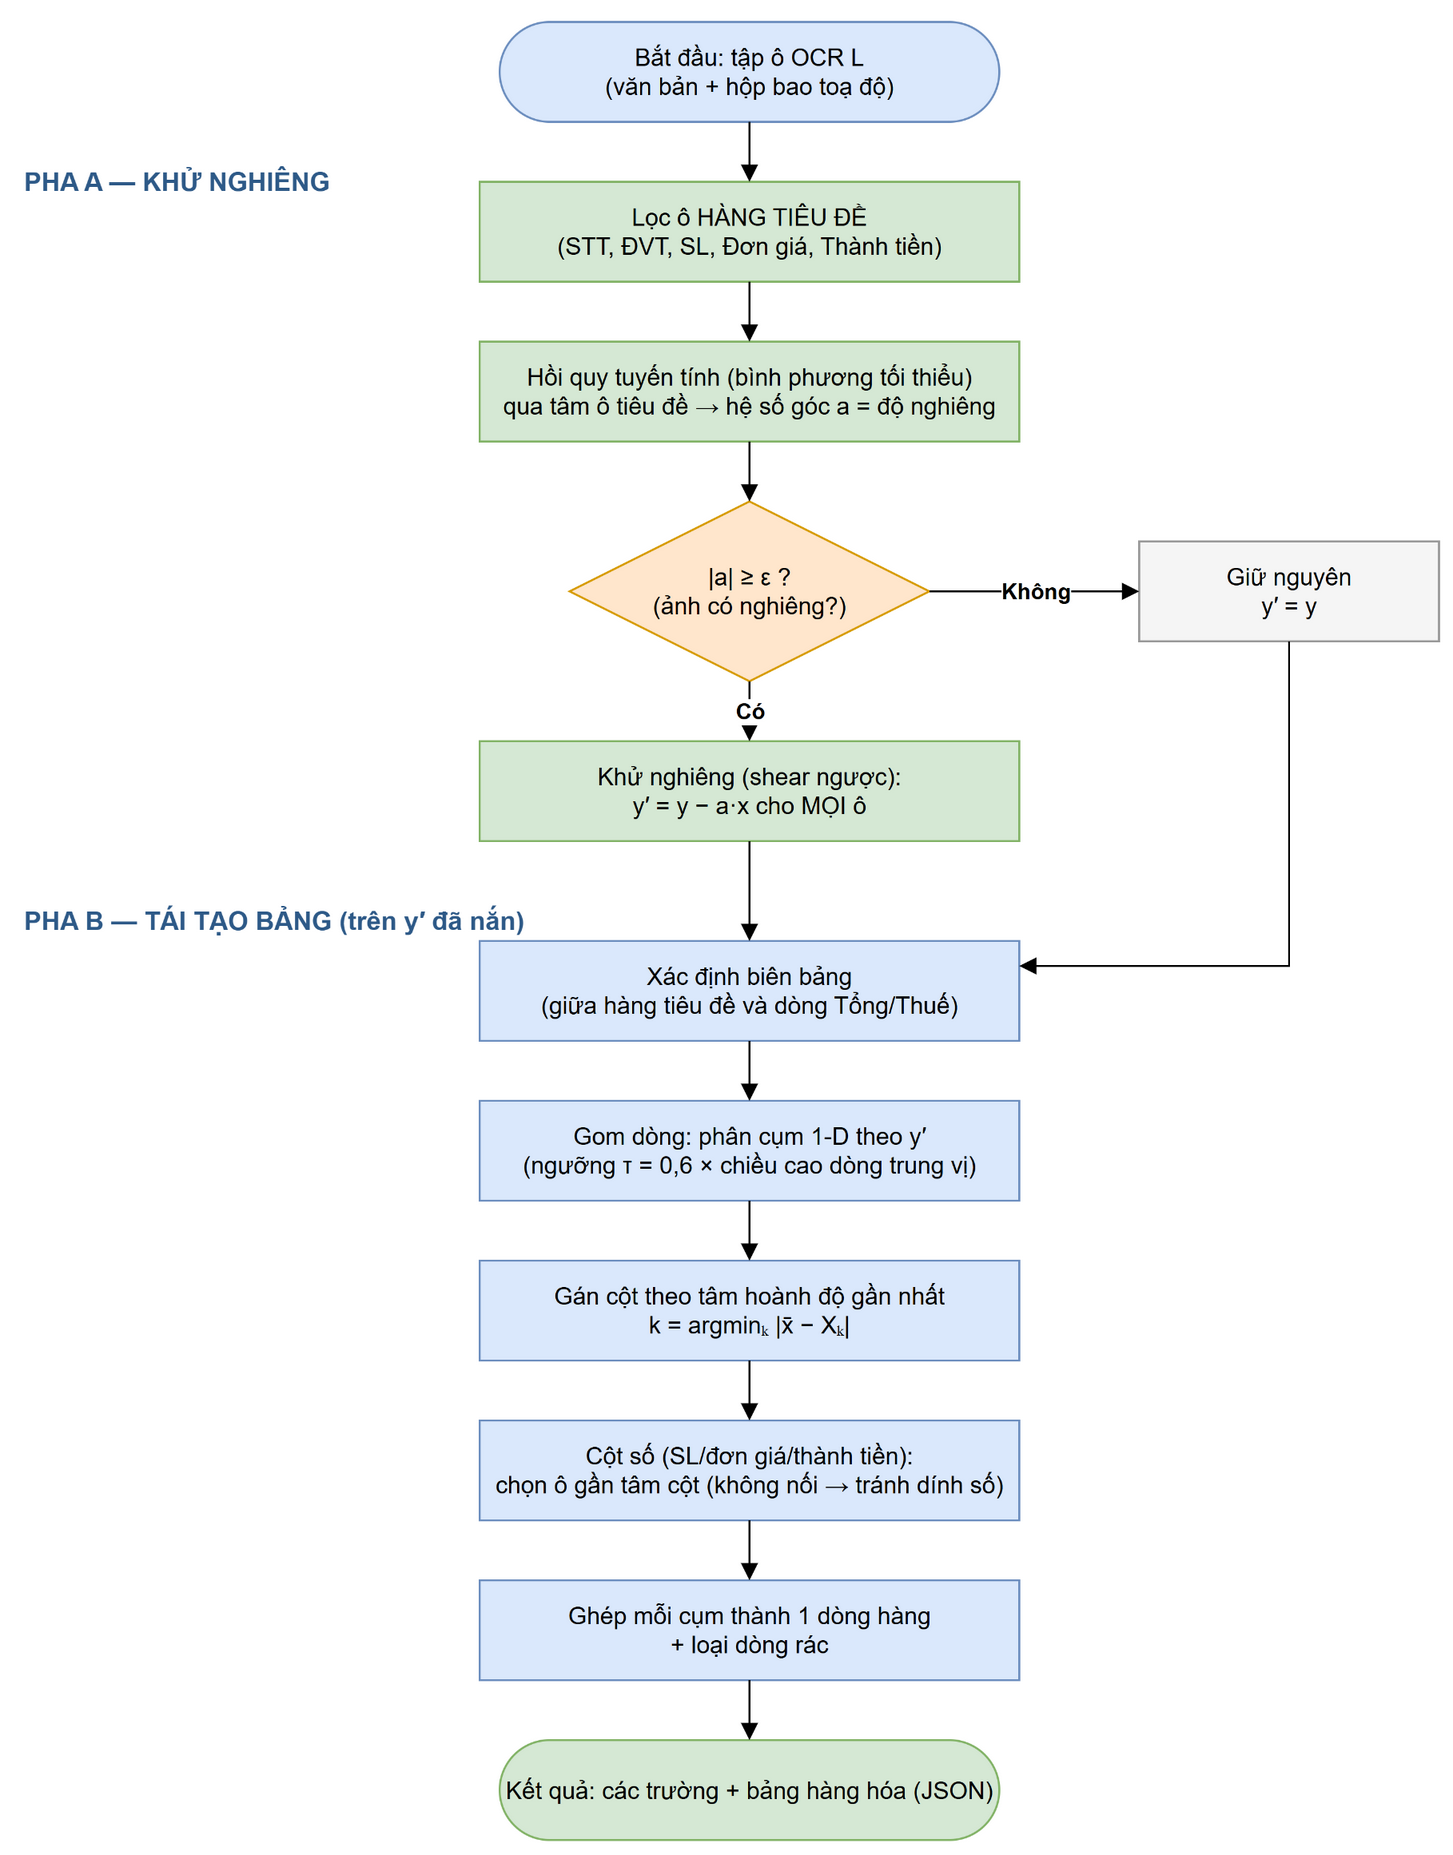
\includegraphics[width=\linewidth,height=0.42\textheight,keepaspectratio]{images/img34.png}
\caption*{\small Hình 4.23. Sơ đồ khối thuật toán bóc tách hóa đơn kháng nghiêng (deskew)}
\addcontentsline{lof}{figure}{Hình 4.23. Sơ đồ khối thuật toán bóc tách hóa đơn kháng nghiêng}
\end{figure}
\subsubsection*{g) Tổng hợp luồng xử lý AI end-to-end}
Hình 4.24 tổng hợp toàn bộ luồng từ ảnh đầu vào đến JSON đầu ra. (1) Đầu vào ảnh hóa đơn (JPG/PNG); (2) tiền xử lý chuẩn hóa RGB; (3) rẽ nhánh theo \texttt{ocrEngine} giữa ba engine tự chủ, đều đi qua lớp Phát hiện rồi Nhận dạng; (4) Phát hiện: CRAFT (vietocr) hoặc DBNet + phân loại góc (paddleocr); (5) Nhận dạng: VietOCR hoặc SVTR\_LCNet tạo danh sách ô OCR (text, box, prob). (6) Hậu xử lý biến ô rời rạc thành dữ liệu có cấu trúc qua năm bước: \textcircled{\scriptsize 1} khử nghiêng ($y' = y - a\cdot x$, bước ĐẦU TIÊN), \textcircled{\scriptsize 2} gom hàng theo $y'$, \textcircled{\scriptsize 3} trích trường bằng nhãn + regex, \textcircled{\scriptsize 4} trích bảng theo tâm cột, \textcircled{\scriptsize 5} chuẩn hóa số và bù tổng. (7) Đầu ra JSON (fields, lineItems, confidence) được backend .NET lưu vào Invoice/InvoiceItem và hiển thị ở màn hình xác nhận.

\begin{figure}[htbp]\centering
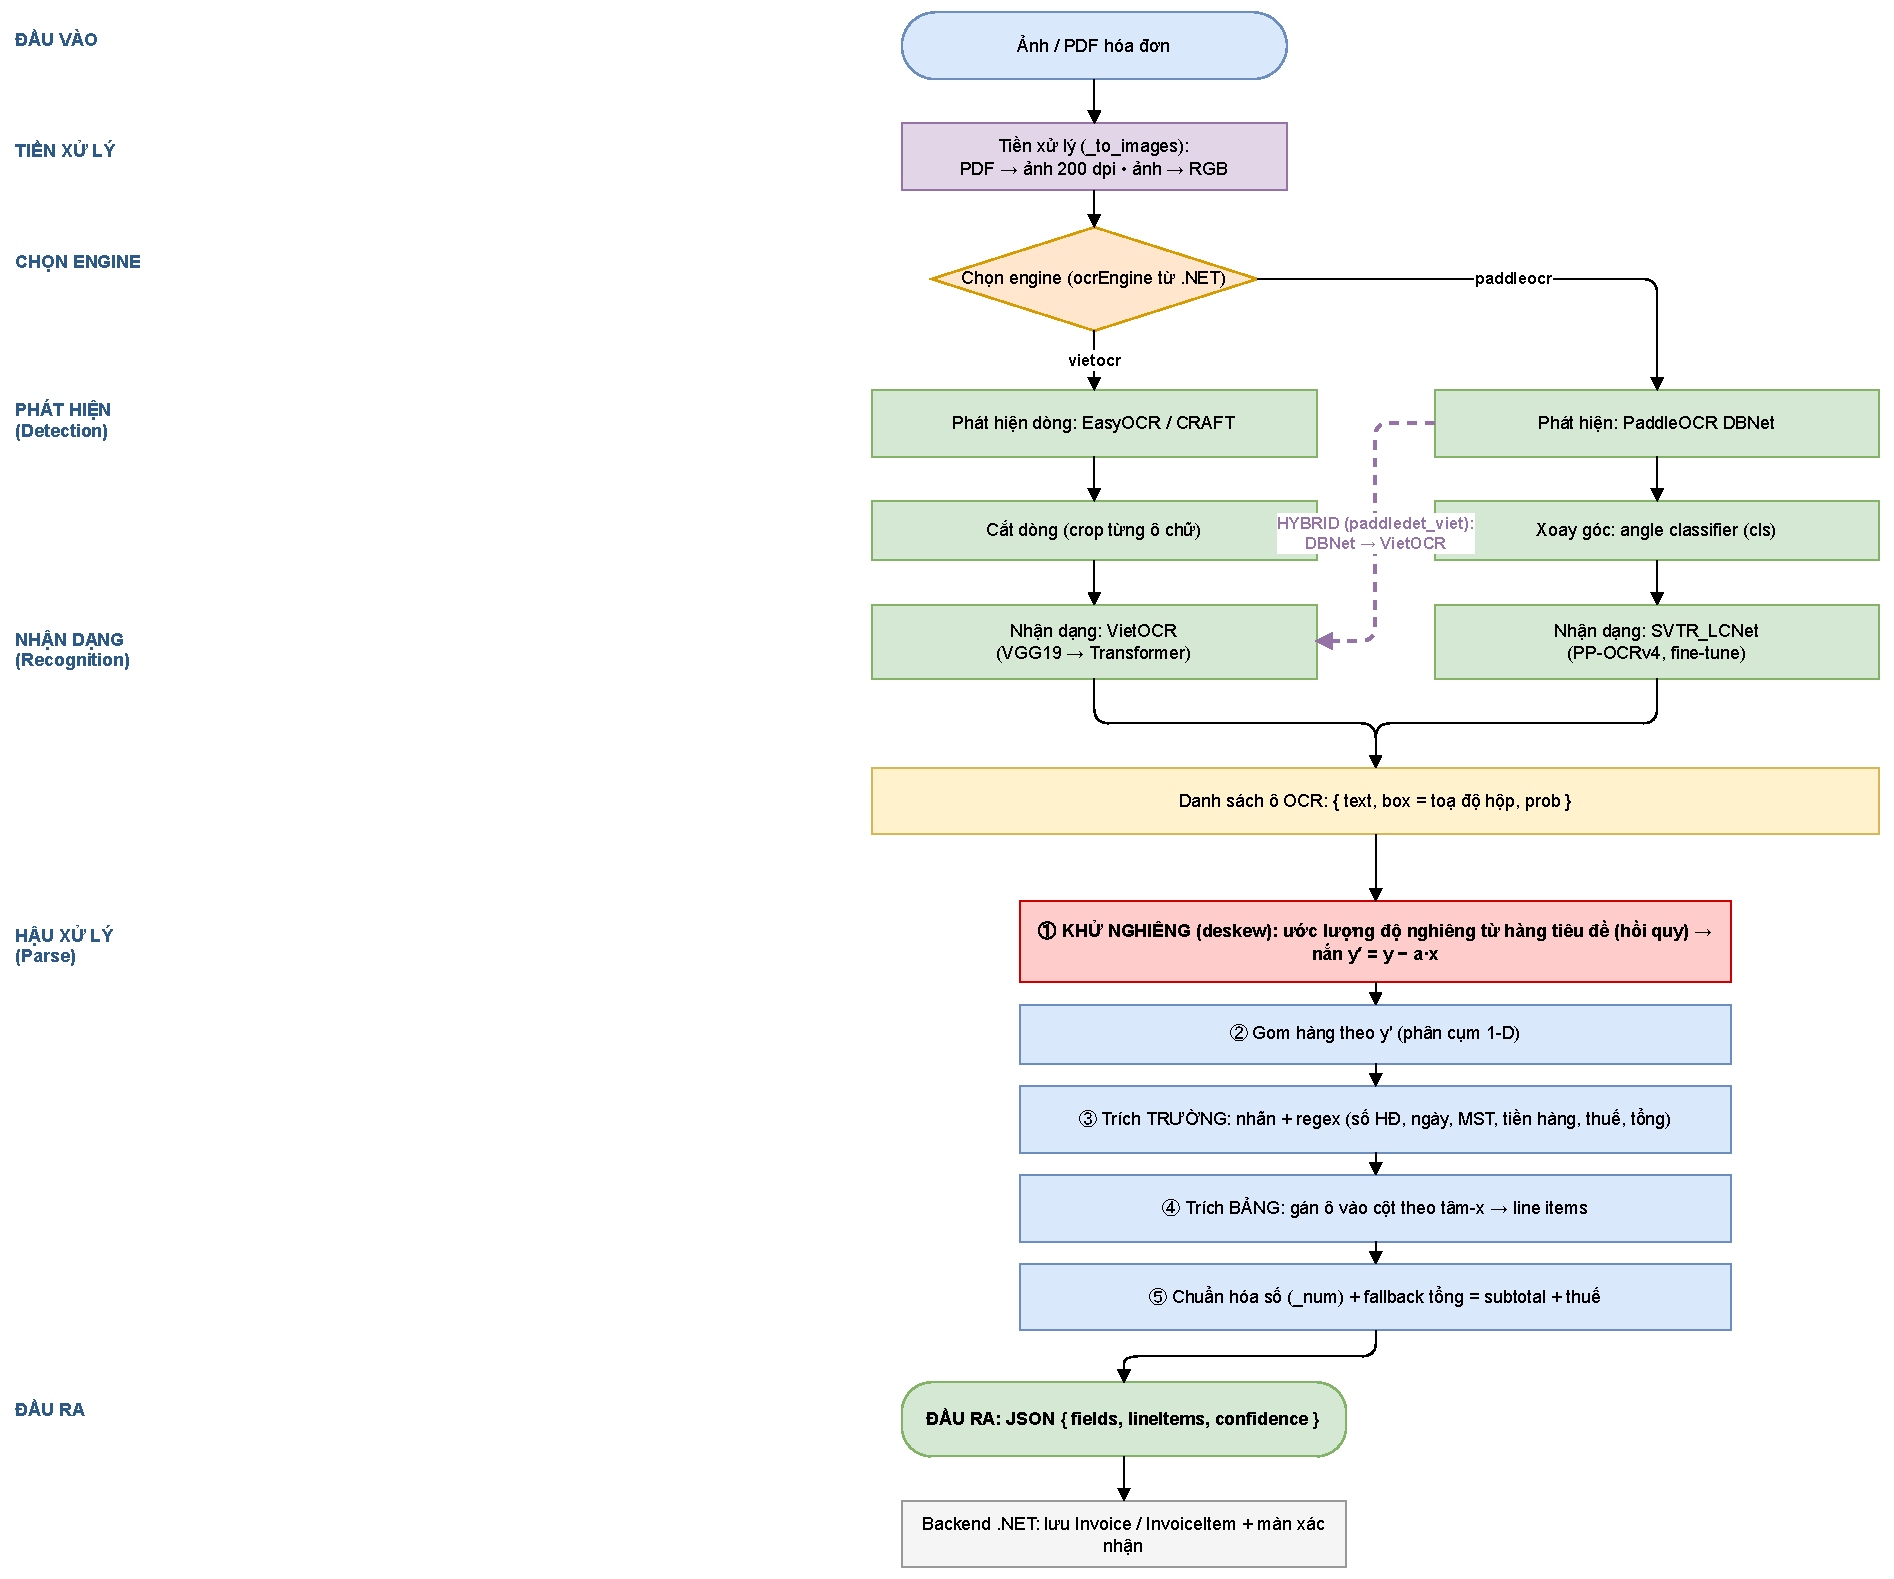
\includegraphics[width=\linewidth,height=0.5\textheight,keepaspectratio]{images/img35.pdf}
\caption*{\small Hình 4.24. Luồng xử lý AI end-to-end của dịch vụ OCR: các lớp xử lý và vị trí bước khử nghiêng}
\addcontentsline{lof}{figure}{Hình 4.24. Luồng xử lý AI end-to-end của dịch vụ OCR}
\end{figure}
\subsubsection*{h) Biến thể hybrid: Paddle DBNet (phát hiện) + VietOCR (nhận dạng)}
\textbf{Ý tưởng \& cơ chế. }VietOCR cho độ chính xác nhận dạng cao nhất, còn DBNet của PaddleOCR (đã fine-tune) phát hiện tốt hơn CRAFT của EasyOCR. Biến thể hybrid (\texttt{paddledet\_viet}) ghép hai điểm mạnh: DBNet phát hiện dòng, sau đó phép biến đổi phối cảnh đưa mỗi vùng (đa giác bốn điểm của DBNet) về ảnh dòng nằm ngang rồi giao VietOCR nhận dạng. Kết quả trả về cùng định dạng danh sách ô nên tái dùng nguyên vẹn bộ hậu xử lý ở mục f, g.

\textbf{Đánh đổi và lựa chọn. }So sánh \texttt{paddleocr} với \texttt{paddledet\_viet} là một ablation giữ nguyên detector, chỉ thay recognizer. Khác biệt của hybrid nằm ở tầng phát hiện: DBNet cắt dòng ổn định hơn CRAFT nên khi chạy end-to-end trên hóa đơn cả trang, hybrid được kỳ vọng vượt pipeline vietocr. Bù lại, hybrid phải nạp đồng thời hai framework (PaddlePaddle + PyTorch) nên tốn bộ nhớ và chậm hơn, triển khai phức tạp hơn PaddleOCR hợp nhất. Vì vậy hệ thống chọn PaddleOCR làm engine mặc định, còn hybrid là tùy chọn phục vụ đối chiếu và tình huống ưu tiên độ chính xác nhận dạng hơn tốc độ.

\phantomsection
\subsection*{4.4.2. Khảo sát các giải pháp AI OCR khác và lý do lựa chọn}
\addcontentsline{toc}{subsection}{4.4.2. Khảo sát các giải pháp AI OCR khác và lý do lựa chọn}
Bóc tách hóa đơn bằng AI là bài toán đã trưởng thành, có nhiều giải pháp thương mại và mã nguồn mở. Trước khi tự xây dựng engine, nhóm đã khảo sát ba nhóm giải pháp phổ biến để làm căn cứ lựa chọn (số liệu giá tham khảo tại thời điểm khảo sát 07/2026); bảng tổng hợp và bảng xếp hạng công khai ở cuối mục.

\textbf{a) Nhóm dịch vụ đám mây (Cloud OCR/IDP API).} Các API trả tiền theo lượt gọi, độ chính xác cao và không phải tự vận hành hạ tầng, nhưng dữ liệu phải gửi ra máy chủ bên thứ ba và chi phí tăng theo sản lượng:
\begin{itemize}[leftmargin=1.4em,itemsep=1pt,topsep=2pt]
  \item \textbf{Google Cloud Vision / Document AI}: giá cơ bản \textasciitilde{}1,5 USD/1.000 trang, bản trích cấu trúc (Document AI) cao hơn nhiều; miễn phí 1.000 đơn vị/tháng.
  \item \textbf{Azure AI Document Intelligence}: có mô hình hóa đơn dựng sẵn (prebuilt-invoice), \textasciitilde{}10 USD/1.000 trang; miễn phí 500 trang/tháng.
  \item \textbf{Amazon Textract}: DetectDocumentText \textasciitilde{}1,5 USD/1.000 trang, AnalyzeDocument (bảng/biểu mẫu) tới \textasciitilde{}65 USD/1.000 trang.
\end{itemize}

\textbf{b) Nhóm SDK thương mại cài tại chỗ.} Tiêu biểu là \textbf{ABBYY FineReader Engine} — bộ SDK OCR lâu đời, độ chính xác cao, chạy được on-premise (bảo mật tốt) nhưng chi phí bản quyền lớn và mô hình đóng, không tùy biến sâu cho hóa đơn tiếng Việt.

\textbf{c) Nhóm mã nguồn mở, tự triển khai.} Miễn phí, chạy offline, tùy biến và fine-tune được:
\begin{itemize}[leftmargin=1.4em,itemsep=1pt,topsep=2pt]
  \item \textbf{Tesseract}: engine mã nguồn mở lâu đời của Google; đọc tài liệu in tốt nhưng yếu với hóa đơn tiếng Việt bố cục phức tạp nếu không huấn luyện lại, và chậm hơn.
  \item \textbf{PaddleOCR} (Hình 4.25): bộ công cụ OCR nhẹ, hợp nhất phát hiện + nhận dạng, hỗ trợ 100+ ngôn ngữ, fine-tune được cả hai tầng, nhanh — đây là engine nhóm chọn, kết hợp thêm \textbf{VietOCR} (recognizer mạnh về dấu tiếng Việt) và bộ phát hiện CRAFT của EasyOCR.
\end{itemize}

\begin{figure}[htbp]\centering
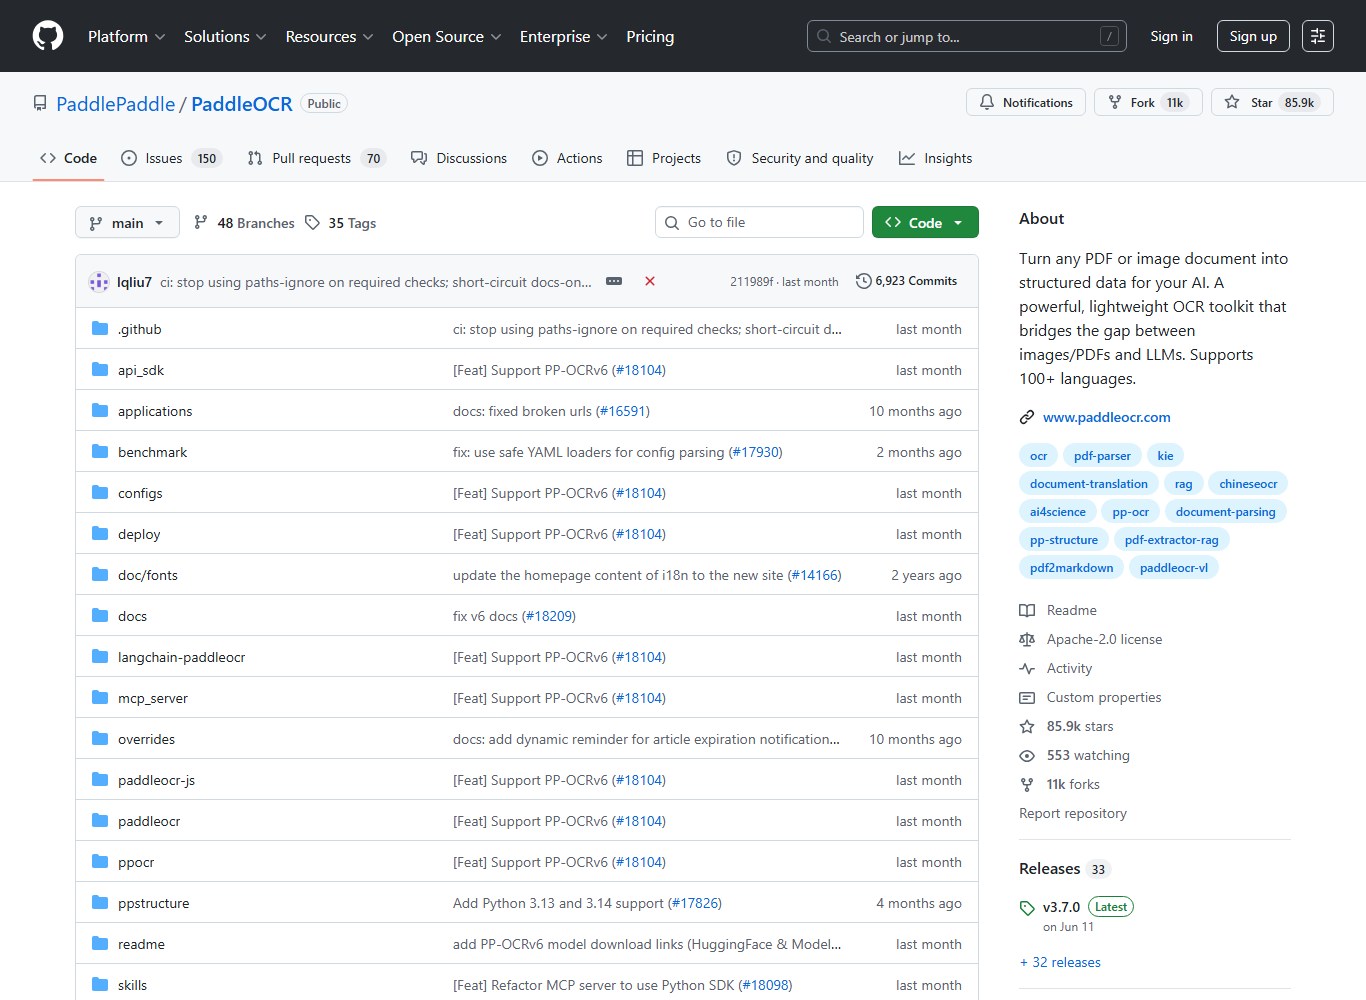
\includegraphics[width=\linewidth,height=0.34\textheight,keepaspectratio]{images/ocr_paddle.png}
\caption*{\small Hình 4.25. PaddleOCR (mã nguồn mở, Apache-2.0, \textasciitilde{}86k sao GitHub) -- engine nhóm lựa chọn}
\addcontentsline{lof}{figure}{Hình 4.25. PaddleOCR (mã nguồn mở) -- engine được chọn}
\end{figure}
\noindent\textit{\small Nguồn: \url{https://github.com/PaddlePaddle/PaddleOCR} (truy cập 07/2026).}

\textbf{Bảng xếp hạng, so sánh các giải pháp.} Nhóm chấm điểm theo các tiêu chí quan trọng với bài toán (đọc hóa đơn tiếng Việt trong hệ quản lý tòa nhà) và với yêu cầu của một đồ án tốt nghiệp:

\begin{landscape}\begin{center}{\footnotesize\singlespacing\renewcommand{\arraystretch}{1.25}
\begin{tabular}{|>{\raggedright\arraybackslash}p{3.1cm}|>{\raggedright\arraybackslash}p{2.3cm}|>{\raggedright\arraybackslash}p{2.6cm}|>{\raggedright\arraybackslash}p{2.6cm}|>{\raggedright\arraybackslash}p{2.5cm}|>{\raggedright\arraybackslash}p{2.5cm}|>{\raggedright\arraybackslash}p{2.4cm}|}
\hline
\textbf{Giải pháp} & \textbf{Loại} & \textbf{Độ chính xác HĐ tiếng Việt} & \textbf{Chi phí} & \textbf{Tự chủ / Offline \& bảo mật} & \textbf{Fine-tune trên dữ liệu riêng} & \textbf{Phù hợp đồ án} \\ \hline
Google Vision / Document AI & Cloud API & Cao & Trả theo lượt (\textasciitilde{}1,5–nhiều USD/1k trang) & Không (gửi HĐ lên cloud) & Hạn chế (không sở hữu model) & Thấp \\ \hline
Azure Document Intelligence & Cloud API & Cao & \textasciitilde{}10 USD/1k trang (invoice) & Không / có container trả phí & Custom model (trả phí) & Thấp \\ \hline
Amazon Textract & Cloud API & Cao & \textasciitilde{}1,5–65 USD/1k trang & Không & Không & Thấp \\ \hline
ABBYY FineReader & SDK thương mại & Cao & Bản quyền lớn & Có (on-prem) & Hạn chế (đóng) & Thấp \\ \hline
Tesseract & Mã nguồn mở & Trung bình–thấp & Miễn phí & Có & Có (khó) & Trung bình \\ \hline
\textbf{PaddleOCR (chọn)} & Mã nguồn mở & \textbf{Cao} (0,893 seq; 65 ms) & Miễn phí & \textbf{Có} & \textbf{Có (det+rec)} & \textbf{Rất phù hợp} \\ \hline
\textbf{VietOCR (chọn)} & Mã nguồn mở & \textbf{Rất cao} (1,000 seq) & Miễn phí & \textbf{Có} & \textbf{Có (rec)} & \textbf{Rất phù hợp} \\ \hline
\end{tabular}}\end{center}\end{landscape}
\noindent\textit{\small Nguồn số liệu giá: trang giá chính thức của Google Cloud Vision, Azure AI Document Intelligence và \url{https://aws.amazon.com/textract/pricing/} (07/2026); số liệu độ chính xác/tốc độ engine lấy từ thực nghiệm của nhóm ở mục 4.4.1.d.}

\textbf{Đối chiếu với bảng xếp hạng AI công khai (OmniDocBench).} Để tăng tính khách quan, nhóm đối chiếu lựa chọn của mình với bảng xếp hạng độc lập, công khai \textbf{OmniDocBench} (CVPR 2025, nhóm OpenDataLab) — benchmark chuẩn cho bài toán bóc tách tài liệu, chấm điểm end-to-end trên nhiều loại tài liệu và cập nhật liên tục cho cả mô hình mã nguồn mở lẫn thương mại. Đáng chú ý, \textbf{PaddleOCR — chính là họ engine đề tài sử dụng — hiện dẫn đầu bảng}: biến thể \texttt{PP-StructureV3} và các mô hình \texttt{PaddleOCR-VL} đạt điểm tổng cao nhất, vượt cả mô hình đa phương thức thương mại như GPT-5.2 hay Gemini~3~Pro. Trích một phần bảng xếp hạng (điểm \emph{Overall}, thang 100, 07/2026):

\begin{center}{\footnotesize\singlespacing\renewcommand{\arraystretch}{1.25}
\begin{tabular}{|c|>{\raggedright\arraybackslash}p{5.0cm}|>{\raggedright\arraybackslash}p{3.4cm}|c|}
\hline
\textbf{Hạng} & \textbf{Mô hình / công cụ} & \textbf{Loại} & \textbf{Overall} \\ \hline
1 & \textbf{PaddleOCR-VL-1.6} \textit{(họ PaddleOCR)} & Mã nguồn mở & \textbf{96,34} \\ \hline
2 & MinerU2.5-Pro & Mã nguồn mở & 95,75 \\ \hline
4 & \textbf{PaddleOCR-VL-1.5} \textit{(họ PaddleOCR)} & Mã nguồn mở & \textbf{94,93} \\ \hline
13 & Gemini 3 Pro \textit{(tham chiếu)} & VLM thương mại & 92,91 \\ \hline
\end{tabular}}\end{center}

\begin{figure}[htbp]\centering
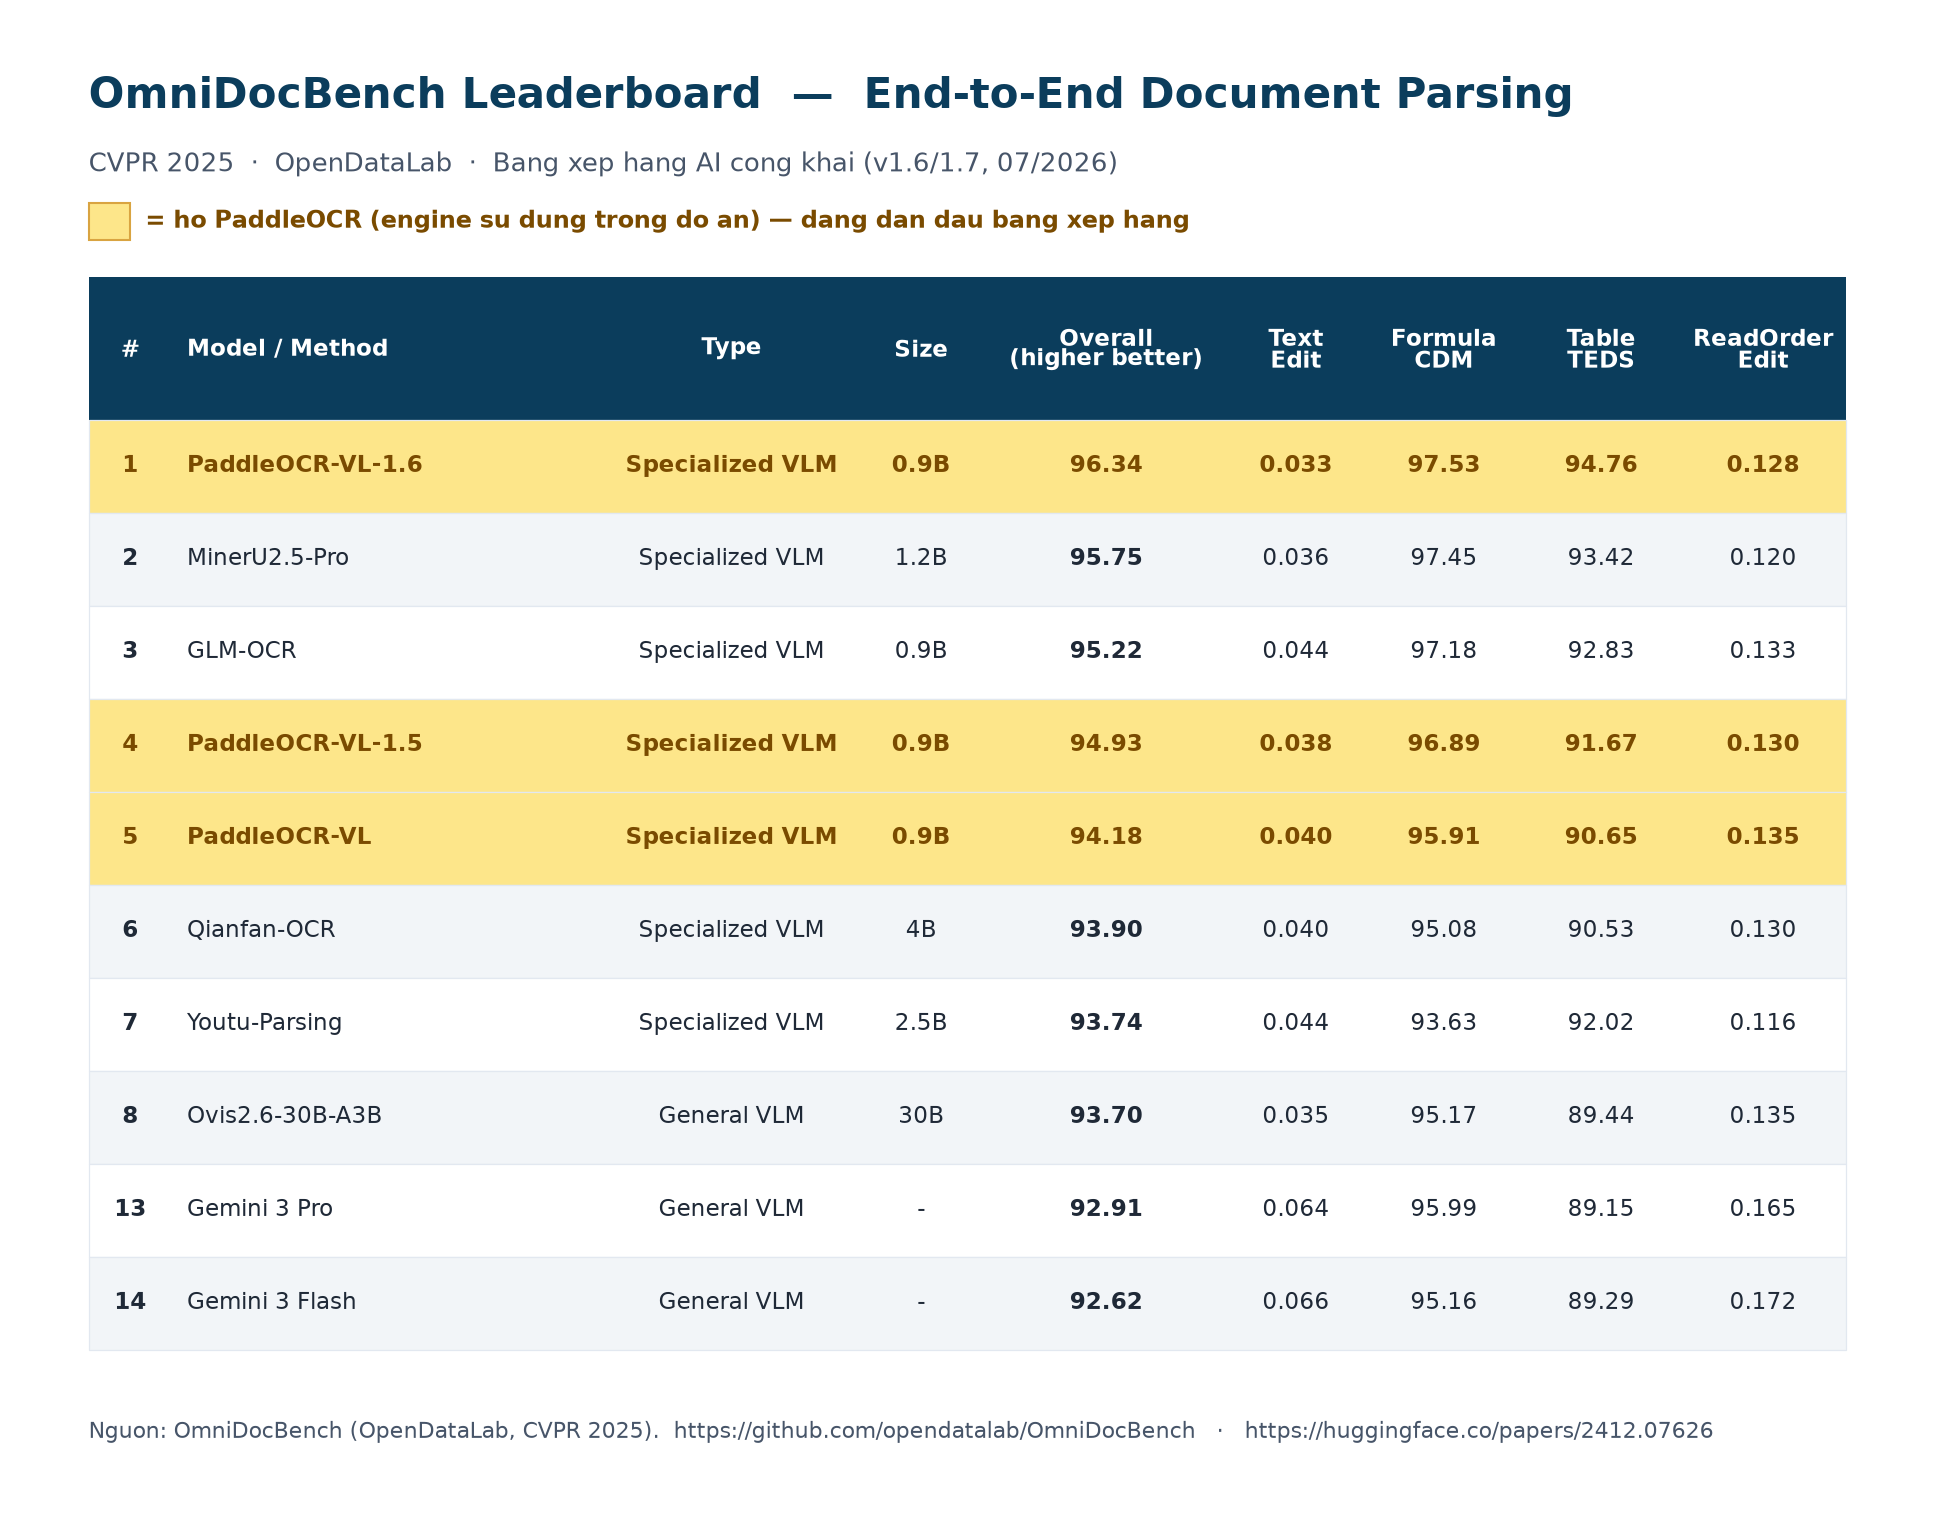
\includegraphics[width=\linewidth,height=0.34\textheight,keepaspectratio]{images/ocr_leaderboard_omnidocbench.png}
\caption*{\small Hình 4.26. Bảng xếp hạng AI công khai OmniDocBench (CVPR 2025) — họ engine PaddleOCR dẫn đầu}
\addcontentsline{lof}{figure}{Hình 4.26. Bảng xếp hạng AI công khai OmniDocBench — PaddleOCR dẫn đầu}
\end{figure}
\noindent\textit{\small Nguồn: OmniDocBench, OpenDataLab (CVPR 2025): \url{https://github.com/opendatalab/OmniDocBench}; \url{https://opendatalab.com/OmniDocBench} (truy cập 07/2026).}

\textbf{Lý do lựa chọn PaddleOCR + VietOCR (tự triển khai).} Trên cơ sở khảo sát, nhóm chọn hướng \emph{tự triển khai mã nguồn mở} thay vì API đám mây hay SDK thương mại, vì: \textbf{(1) Bảo mật} — hóa đơn chứa thông tin tài chính–thuế nhạy cảm, giải pháp tự triển khai chạy offline, dữ liệu không rời khỏi hệ thống; \textbf{(2) Chi phí} — miễn phí bản quyền, không phí theo lượt gọi (API đám mây \textasciitilde{}1,5–65 USD/1.000 trang); \textbf{(3) Fine-tune được trên dữ liệu tiếng Việt} — nhóm tự sinh dataset và fine-tune đạt 99,64\% (PaddleOCR) và 100\% (VietOCR), điều mà API/SDK đóng không cho phép; \textbf{(4) Chủ động}, không lệ thuộc Internet hay vendor lock-in; \textbf{(5) Đúng tinh thần đồ án} — thể hiện năng lực xây dựng, huấn luyện và đánh giá mô hình AI thay vì chỉ gọi dịch vụ có sẵn. Tóm lại, các giải pháp đám mây/thương mại chính xác và tiện nhưng đánh đổi chi phí, quyền riêng tư và khả năng tùy biến; hướng tự triển khai PaddleOCR + VietOCR đáp ứng tốt nhất các tiêu chí của đề tài.

\phantomsection
